\section{背景}
\label{sec:background}

\begin{figure}[t!]
    \centering
    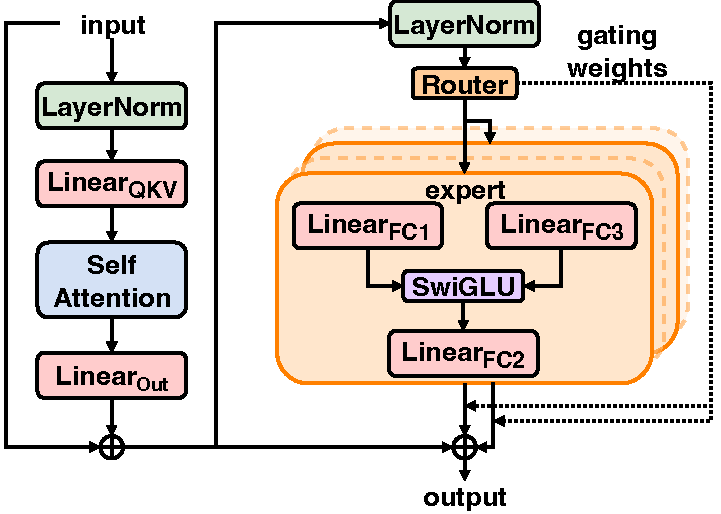
\includegraphics[width=0.65\linewidth]{figures/moe_intro.pdf}
    \vspace{-0.15in}
    \caption{专家混合（MoE）层。}
    \vspace{-0.1in}
    \label{fig:moe_intro}
\end{figure}

\subsection{面向 Transformer 的专家混合}

专家混合（MoE）机制是一种先进方法，旨在提升 Transformer~\cite{vaswani2017attention} 模型的性能；Transformer 在 LLM 领域中正变得日益关键~\cite{jiang2024mixtral, chowdhery2023palm, dbrx, liu2024deepseekv3}。MoE 通过在前馈网络（FFN）组件中集成多个专家网络来扩展 Transformer 架构。如 图~\ref{fig:moe_intro} 所示，MoE 模型会根据输入 token 的特征，将其动态路由到最相关的专家。该路由由可训练的 gating 机制管理，为每个 token 选择最合适的专家。由于每个输入只激活一部分专家，这种架构创新使 MoE 模型能够扩大容量，而不会使推理成本按比例增长。
% It offers a more flexible and efficient way to improve model performance beyond simply increasing the size of the network.

\subsection{大规模 LLM 训练}

在数万张 GPU 上大规模训练大语言模型是一项复杂的系统工程挑战，需要多种系统技术。为了分布训练负载，必须结合数据并行、张量并行和流水线并行等并行策略~\cite{shoeybi2019megatron, rasley2020deepspeed, jiang2024megascale}，因为每种方法都有局限，单独依赖某一种方法无法有效扩展。

\parabf{数据并行} 将训练数据均匀分布到所有设备上，每个设备都复制模型参数和优化器状态。为了在每次训练迭代后同步参数，数据并行会执行 all-reduce 通信操作。Zero Redundancy Optimizer（ZeRO）~\cite{rajbhandari2020zero} 通过在所有参与设备之间分布模型状态来改进数据并行。ZeRO 分为三个递进阶段，每个阶段都进一步节省内存，但代价是通信开销增加。

\parabf{张量并行} 将计算密集型张量操作分布到多个设备上，从而实现并行计算并显著加速训练过程。具体的划分策略以及模型内部算子之间的依赖关系，决定了张量并行可能需要收集被切分的输入（all-gather）或合并输出（reduce-scatter）。在 LLM 训练中，LayerNorm 和 Dropout 等算子虽然计算不密集，却需要大量激活内存。为解决这一问题，研究者提出了称为 \textbf{序列并行} 的张量并行变体~\cite{korthikanti2023reducing}，沿序列长度维度划分这些算子。对于长上下文训练，一些工作~\cite{shoeybi2019megatron, jacobs2023deepspeed, context_parallelism} 将序列并行或张量并行应用到自注意力中的不同算子。图~\ref{fig:background:attention_parallelism} 展示了注意力的主流并行策略，即张量并行、序列并行和上下文并行（TP、SP 和 CP），我们将在 \S\ref{sec:design:parallelism:sp_attention} 中分析它们。

\begin{figure}[t!]
    \centering
    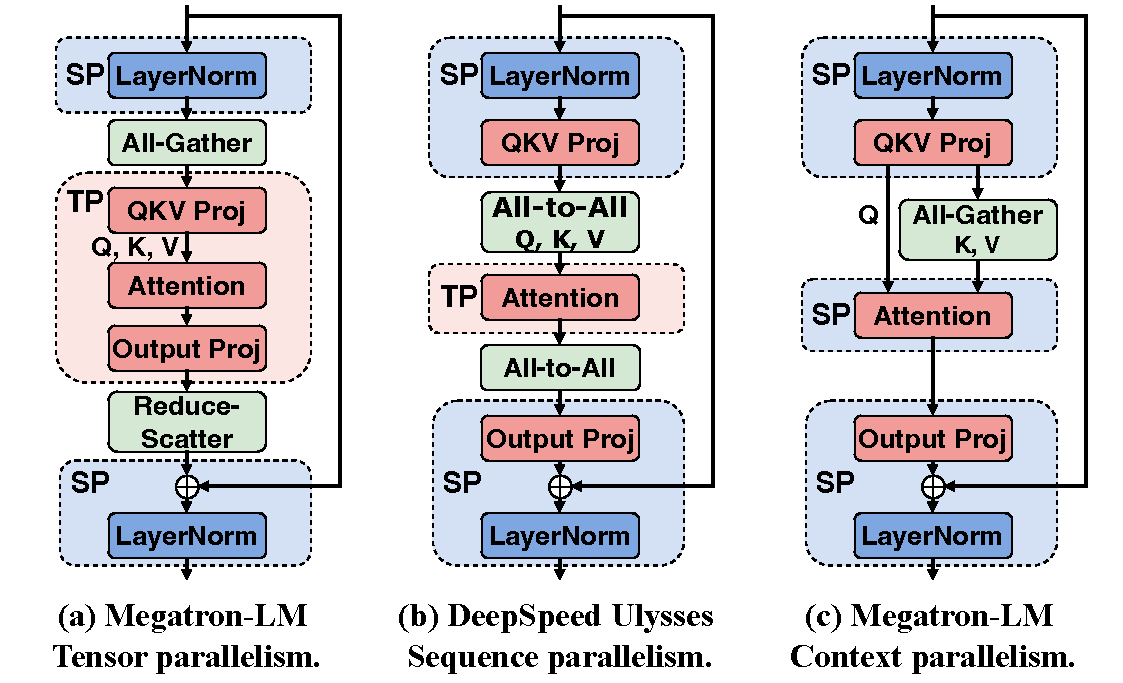
\includegraphics[width=\linewidth]{figures/megascale-moe-attention-parallelism.pdf}
    \vspace{-0.3in}
    \caption{自注意力的不同并行策略。“TP”表示沿隐藏维度划分，“SP”表示沿序列长度维度划分。}
    \vspace{-0.1in}
    \label{fig:background:attention_parallelism}
\end{figure}

\parabf{流水线并行} 通过将模型层划分为不同阶段并在不同设备上处理来提升效率，从而实现流水线执行。为此，每个 batch 会被拆分为多个 micro-batch。为了减少流水线气泡，已有多种调度策略被提出，例如 GPipe~\cite{huang2019gpipe}、PipeDream 1F1B~\cite{narayanan2019pipedream} 和 Interleaved 1F1B~\cite{narayanan2021efficient} 等。Megatron-LM 采用 Interleaved 1F1B 流水线调度，将一个设备上的每个阶段进一步划分为多个虚拟阶段，以降低流水线气泡率。

\parabf{专家并行} 专门用于训练 MoE 模型，它将专家分布到多个设备上，从而缓解内存压力并支持并行处理。为了高效地将 token 分配给合适的专家并取回其输出，通常会使用 all-to-all 通信。

\iffalse

\begin{table*}[t!]
    \centering
    \resizebox{\linewidth}{!} {
        \begin{tabular}{c|c|c|c|c|c|c}
            \hline
            \hline
            \multirow{2}{*}{\begin{tabular}[c]{@{}c@{}}Parallelism Strategy\end{tabular}} & \multicolumn{3}{c|}{Partitioning Dimension} & \multirow{2}{*}{\begin{tabular}[c]{@{}c@{}}Communication\\ Operation\end{tabular}} & \multirow{2}{*}{\begin{tabular}[c]{@{}c@{}}Communication\\ Volume\end{tabular}} & \multirow{2}{*}{\begin{tabular}[c]{@{}c@{}}Attention \\Parameters\end{tabular}}\\
            \cline{2-4}
            & $ \text{Linear}_{\text{QKV}} $ & Attention & $ \text{Linear}_{\text{Out}} $ & & & \\
            \hline
            Tensor Parallelism (TP)~\cite{shoeybi2019megatron} & H & H & H & All-Gather+Reduce-Scatter & $2bsh(n-1)/n$ & Partitioned \\
            Ulysses Sequence Parallelism (SP)~\cite{jacobs2023deepspeed} & S & H & S & All-to-All QKV\&Output & $2bsh(n-1)/n \times (2+2/m)/n$ & Replicated \\
            Context Parallelism (CP)~\cite{context_parallelism} & S & S & S & All-Gather KV & $2bsh(n-1)/n \times 2/m$ & Replicated \\
            \hline
            \hline
        \end{tabular}
    }
    % \vspace{-0.1in}
    \caption{Different parallelism strategies for self-attention. "H" denotes partitioning along the dimension of hidden size, while "S" denotes partitioning along the dimension of sequence length.}
    \vspace{-0.1in}
    \label{tab:background:parallelism}
\end{table*}
\fi
